\documentclass[]{article}
\usepackage{lmodern}
\usepackage{amssymb,amsmath}
\usepackage{ifxetex,ifluatex}
\usepackage{fixltx2e} % provides \textsubscript
\ifnum 0\ifxetex 1\fi\ifluatex 1\fi=0 % if pdftex
  \usepackage[T1]{fontenc}
  \usepackage[utf8]{inputenc}
\else % if luatex or xelatex
  \ifxetex
    \usepackage{mathspec}
    \usepackage{xltxtra,xunicode}
  \else
    \usepackage{fontspec}
  \fi
  \defaultfontfeatures{Mapping=tex-text,Scale=MatchLowercase}
  \newcommand{\euro}{€}
\fi
% use upquote if available, for straight quotes in verbatim environments
\IfFileExists{upquote.sty}{\usepackage{upquote}}{}
% use microtype if available
\IfFileExists{microtype.sty}{%
\usepackage{microtype}
\UseMicrotypeSet[protrusion]{basicmath} % disable protrusion for tt fonts
}{}
\usepackage[margin=1in]{geometry}
\ifxetex
  \usepackage[setpagesize=false, % page size defined by xetex
              unicode=false, % unicode breaks when used with xetex
              xetex]{hyperref}
\else
  \usepackage[unicode=true]{hyperref}
\fi
\hypersetup{breaklinks=true,
            bookmarks=true,
            pdfauthor={Jan Winter},
            pdftitle={caRpools Installation Guide},
            colorlinks=true,
            citecolor=blue,
            urlcolor=blue,
            linkcolor=magenta,
            pdfborder={0 0 0}}
\urlstyle{same}  % don't use monospace font for urls
\usepackage{graphicx,grffile}
\makeatletter
\def\maxwidth{\ifdim\Gin@nat@width>\linewidth\linewidth\else\Gin@nat@width\fi}
\def\maxheight{\ifdim\Gin@nat@height>\textheight\textheight\else\Gin@nat@height\fi}
\makeatother
% Scale images if necessary, so that they will not overflow the page
% margins by default, and it is still possible to overwrite the defaults
% using explicit options in \includegraphics[width, height, ...]{}
\setkeys{Gin}{width=\maxwidth,height=\maxheight,keepaspectratio}
\setlength{\parindent}{0pt}
\setlength{\parskip}{6pt plus 2pt minus 1pt}
\setlength{\emergencystretch}{3em}  % prevent overfull lines
\providecommand{\tightlist}{%
  \setlength{\itemsep}{0pt}\setlength{\parskip}{0pt}}
\setcounter{secnumdepth}{5}

%%% Use protect on footnotes to avoid problems with footnotes in titles
\let\rmarkdownfootnote\footnote%
\def\footnote{\protect\rmarkdownfootnote}

%%% Change title format to be more compact
\usepackage{titling}

% Create subtitle command for use in maketitle
\newcommand{\subtitle}[1]{
  \posttitle{
    \begin{center}\large#1\end{center}
    }
}

\setlength{\droptitle}{-2em}
  \title{caRpools Installation Guide}
  \pretitle{\vspace{\droptitle}\centering\huge}
  \posttitle{\par}
  \author{Jan Winter}
  \preauthor{\centering\large\emph}
  \postauthor{\par}
  \date{}
  \predate{}\postdate{}


% Redefines (sub)paragraphs to behave more like sections
\ifx\paragraph\undefined\else
\let\oldparagraph\paragraph
\renewcommand{\paragraph}[1]{\oldparagraph{#1}\mbox{}}
\fi
\ifx\subparagraph\undefined\else
\let\oldsubparagraph\subparagraph
\renewcommand{\subparagraph}[1]{\oldsubparagraph{#1}\mbox{}}
\fi

\begin{document}
\maketitle

{
\hypersetup{linkcolor=black}
\setcounter{tocdepth}{3}
\tableofcontents
}
\newpage

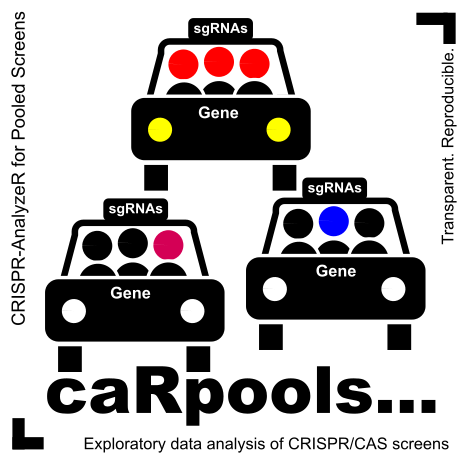
\includegraphics{./pictures/CaRpools.png}

\newpage

\section{Requirements and
Installation}\label{requirements-and-installation}

\subsection{Download caRpools}\label{download-carpools}

CaRpools is avaible as an R package \textbf{caRpools} without the
scripts and template files.\\
The complete package with the PERL scripts and all template files can be
obtained from \href{https://github.com/boutroslab/carpools}{Github}
(\url{https://github.com/boutroslab/carpools}) and our website
\href{http://www.crispr-analyzer.org}{crispr-analyzer.de}.

We recommend to download the template files and Scripts from Github and
install caRpools in R using the package installer
`install.packages(``caRpools'').

\subsection{Virtual Box Image - The FAST-track -
RECOMMENDED}\label{virtual-box-image---the-fast-track---recommended}

We also included a VirtualBox Image that already includes all necessary
software and package files. \textbf{In this case no additional software
except for Virtual Box 5 needs to be installed.}

\textbf{We recommend using the Virtual Box image as it provides a fast,
easy and convenient way of using caRpools for the generation of reports
for every user.}

You just need to install VirtualBox 5 from the
\href{https://www.virtualbox.org}{Website}.

\textbf{Please follow the manual}
\href{https://github.com/boutroslab/caRpools/blob/master/docs/CaRpools-SHORTGUIDE-VirtualBox.Rmd}{here}

You can then download the caRpools virtual box image from our website
\href{http://www.crispr-analyzer.de}{crispr-analyzer.de} or
\href{https://github.com/boutroslab/carpools}{Github}
(\url{https://github.com/boutroslab/carpools}).

\subsubsection{How to use the Virtual Box
caRpools}\label{how-to-use-the-virtual-box-carpools}

\textbf{Please follow the manual}
\href{https://github.com/boutroslab/caRpools/blob/master/docs/CaRpools-SHORTGUIDE-VirtualBox.Rmd}{here}\\
or the \textbf{CaRpools-SHORTGUIDE-VirtualBox.pdf} /
\textbf{CaRpools-SHORTGUIDE-VirtualBox.html}

\subsection{Hardware Requirements}\label{hardware-requirements}

For CRISPR-Libraries of 12 K size (12K sgRNAs), caRpools will work on
any laptop/PC with at least 4GB of RAM and a modern dual-core CPU.\\
CRISPR-Libraries with a size of more than 100 K (100 K sgRNAs) run best
with at least 8 GB of RAM.

\subsection{Software Requirements}\label{software-requirements}

CaRpools was tested on MacOSX Yosemite and Ubuntu 14.04 LTS.\\
However, it should work on any operating system that fulfills the
software requirments.

The following software needs to be installed:

\begin{itemize}
\tightlist
\item
  PERL 5
\item
  Bowtie2 2.2.0 or higher
  \href{http://bowtie-bio.sourceforge.net/bowtie2/index.shtml}{Website}
\item
  MAGeCK 0.51 (password protected download)
  \href{http://sourceforge.net/p/mageck/wiki/Home/}{Website}
\item
  TexLive \href{https://www.tug.org/texlive/}{Website}
\item
  pdflatex
\item
  xelatex
\item
  R 3.2.0 or higher \href{https://www.r-project.org/}{Website}
\item
  Pandoc 1.15.0.6 \href{http://www.http://pandoc.org/}{Website}
\item
  R-Studio \href{http://www.rstudio.com}{Website} (GUI)
\end{itemize}

The following \textbf{R packages} need be installed (can be done via
\texttt{load.packages()}):

\begin{itemize}
\tightlist
\item
  Bioconductor Basics

  \begin{itemize}
  \tightlist
  \item
    BiocInstaller \textgreater{}= 1.18.3
  \item
    BiocGenerics \textgreater{}= 0.14.0
  \end{itemize}
\item
  \textbf{biomaRt \textgreater{}=2.24.0}
\item
  seqinr \textgreater{}= 3.1-3
\item
  xlsx \textgreater{}= 0.5.7
\item
  rJava \textgreater{}= 0.9.6
\item
  xlsxjars \textgreater{}= 0.6.1
\item
  stringi \textgreater{}= 0.5
\item
  scatterplot3d \textgreater{}= 0.3
\item
  MESS \textgreater{}= 0.3
\item
  DESeq2 \textgreater{}= 1.8.1
\item
  rmarkdown \textgreater{}= 0.7
\item
  knitr \textgreater{}= 1.10.5
\item
  VennDiagram \textgreater{}= 1.6.9
\item
  sm \textgreater{}= 2.2
\end{itemize}

\subsection{BiomaRt and Annotation
Requirements}\label{biomart-and-annotation-requirements}

\textbf{Please note that for any annotation, biomaRt needs full access
to the internet.} In case of incorrect proxy settings, the report
generation will fail with a biomaRt error.\\
This means that if any proxy server is used, this has to be configured
before using the CRISPR-Analyzer as described in the following articles:

\begin{itemize}
\tightlist
\item
  \href{http://www.bioconductor.org/packages/release/bioc/vignettes/biomaRt/inst/doc/biomaRt.pdf}{BiomaRt
  vignette}
\item
  \href{https://support.rstudio.com/hc/en-us/articles/200488488-Configuring-R-to-Use-an-HTTP-Proxy}{Setting
  up proxy in R-Studio}
\item
  \href{http://stackoverflow.com/questions/6467277/proxy-setting-for-r}{Setting
  up proxy in R, Stackoverflow}
\item
  \href{http://askubuntu.com/questions/572722/setting-up-the-proxy-for-rstudio}{Setting
  up Proxy for R/R-Studio in Ubuntu}
\item
  \href{https://bhoom.wordpress.com/2013/05/27/configuring-r-to-use-an-http-proxy-faq-knowledge-base-rstudio-support/}{Configuration
  of Proxy for R}
\end{itemize}

\subsection{Installation Procedure}\label{installation-procedure}

Install all software listed above according to the installation
information stated on the software website.\\
All neccesarry R packages can be installed automatically by
\texttt{load.packages()} within R or R-Studio.

See \href{http://www.r-bloggers.com/installing-r-packages/}{Install R
packages} or \href{https://www.youtube.com/watch?v=u1r5XTqrCTQ}{Install
R packages with RStudio}.

\end{document}
